\chapter{Cybersecurity Design}
The aim of cybersecurity design is to discover or instantiate:
axioms, assumptions, and enforced rules which enable us to
prove that the objectives are true.
some intermediate propositions that we also wish to prove.

\section{Introduction}\label{introsec} \thispagestyle{empty}
Cybersecurity is essentially the enforcing of the rules(mandatory objectives and their conditions) required by the stakeholders of the system under consideration.  The collection of cybersecurity rules forms a graph, in which the vertices represent cybersecurity rules, and the edges represent {\em inference}, in the sense that the collection of vertices with edges {\em terminating} at a certain vertex, $V$ for example, correspond to the set of rules which are sufficient to prove the rule corresponding to $V$. This representation of cybersecurity provides a way to develop cybersecurity architecture\cite{Rerup2018}. These diagrams can also be used in security design, as a way to validate security designs, for documentation, and as a way to visualise and develop alternative designs.

%\section{Knowledge Graphs for cybersecurity}
Cybersecurity systems have used Knowledge Graphs (KG) to store and  retrieve data  to make decisions about cyber-attacks 
\iffalse 
We believe that improving the base cyber threat intelligence representation will help improve the overall quality and performance of systems. The dependence of various cybersecurity informatics systems on various knowledge representation schemes makes it imperative that we develop systems that improve these representations. In some cases, a knowledge graph can have incorrect relationships between two cybersecurity entities, or may not even assert a relationship or a few missing relationships. In such a case, we can say that there are a few missing of relationships. we improve knowledge graphs by validating relationships and asserting values for missing relationships \fi \cite{pingle2019relext,jia2018practical, ghose2019multimodal, deng2019knowledge}. Graphical representation of logical or structural properties of computer systems is a well-established practice in computer science \cite{engelen2010integrating}. Inference graphs, as introduced and explained in this paper, provide a graphical representation of cybersecurity architecture.

\subsection{Objectives of this research}

The aim of this research is to develop concepts and tools which assist
cybersecurity professionals to define the security objectives of their
systems, the rules which enforce this security, and the reasoning
behind the choice of these rules. The concepts and tools we propose
and illustrate in this paper will be shown to be sufficient to record
and analyse these rules, both the objectives and the rules which are
enforced, and to ensure that there are no logical flaws in the system
which has been designed. Note that we assume our cybersecurity objectives include
the control of all important risks. 

{\em In Example 1 of Section \ref{examplesec},
we see how a key design objective is achieved rigorously by a clever decision
which emerges from the use the cybersecurity inference graph of this system.
Example 2 is based on a cybersecurity weakness in a web service administered 
by one of the authors, which was analysed and solved previously \cite{exptsandproofs}
so in this case the inference graph is used to illustrate the proofs which were developed then.
In Example 3, finding the correct proofs was a complicated task which was
facilitated by the use of the inference graph of rules and objectives of the system.}



\subsection{Stakeholder Analysis}

\subsection{Stakeholder Analysis}
Stakeholder analysis \cite{exptsandproofs,project2018guide,rose2013guide} begins by identifying those who influence or who are influenced by decisions or outcomes of the system. There are several ways to classify stakeholders  some of which depend on their threat potential. 

As set out in \cite{exptsandproofs}, the most important reason for a careful stakeholder analysis, from the point of view of this paper, is that if we are able to identify a sufficient set of rules to ensure the willing participation of each stakeholder, and if we can enforce these rules, then the system is self-evidently secure.  Through experience, stakeholders may, during the lifetime of a system, discover that there are rules which were not initially obvious and that need to be added to their required rule set. This should not inhibit us from attempting to identify as complete as possible a set of stakeholder rules. Furthermore, if sufficient care is taken with stakeholder analysis, discoveries of missing rules should be infrequent.

\iffalse
\subsection{Commonsense security}
It is known
\cite{cardenas2009challenges, teufel2018cybersecurity, croasdell2019transnational},
that the human dimension in security management is the most important one. Therefore,
awareness management is a key factor. For example, attackers will exploit
any machines that are not updated since an OS flaw was revealed. Therefore, OS updates must be 
installed as soon as possible after update release. Misconfiguration of 
applications or services is another of key source of vulnerabilities.
Device security can be an important issue, especially when staff are 
able to make use of their own network-connected devices.

Poor password practices of staff can create significant vulnerability, 
hence, password management systems -- which enable users to securely manage
their passwords, may be advisable. 
Vulnerability management can increase security by recognising
and reporting suspicious activity dynamically\cite{grawemeyer2011using,jenkins2014improving}.

Inference graphs are relevant to all these issues because they enable
us to create a diagram which shows the dependence of our objectives
(or risks), on the assumptions we make about human behaviour, 
the conditions which we enforce, and the configuration (or mis-configuration)
of component sub-systems.
\fi

\subsection{The Netml system}
Netml is a cloud-based system developed by the University of Southern Queensland and 
City University of Hong Kong. It is used by students to analyse,  design, and simulate networks
\cite{addie2006netml,addie2011netml}. It is freely available for use (in the cloud) at \verb|https://netml.org|.
%
The Netml system is used in this research to create and modify
inference graphs.

A tool which enables graphical editing of inference graphs is essential because 
the layout of an inference graph can improve its clarity and usefulness considerably,
and the only practical way to develop this layout is by manual editing.
In addition, the tools developed in this research, which are described in Section \ref{softwaresec},
may be used via the most recent version of the public Netml server.

Section \ref{inferencesec} defines and explains the concept of an inference graph.
Section \ref{examplesec} uses three examples to illustrate their use. Section \ref{softwaresec}
describes the software tools which have been developed to enable inference
graphs to be readily developed and managed. Finally, Section \ref{concsec}
presents conclusions. A sample of the software which has been developed is presented in the appendix.

 
\section{Inference graphs}\label{inferencesec}
An inference graph shows the relationship of {\em inference} (what implies what)
which applies between the different cybersecurity rules which apply in a system.
Examples of inference graphs are shown in Figures \ref{parcelboxrules} 
and \ref{certificaterulesgraph}. These will be explained in Section \ref{examplesec}.

The following types of rules arise in cybersecurity analysis:
{\em objective}, {\em enforced rule}, {\em axiom}, {\em proposition}, and {\em assumption}.
An objective is a rule which is required to be true at all times.
An enforced rule is a condition which it is possible to enforce,
and which it has been decided to enforce, by technical means.
For example, access to many systems is only provided if a user is able
to enter a valid username and password.

An axiom is a condition which is held to be true {\em a priori};
an assumption is a condition which we {\em choose} to believe.
For example, under some conditions we assume that users do not reveal their
password to other users.
A proposition is a rule or statement which we define in order
to express a useful stage of reasoning.

An {\em edge} in an inference graph connects each of the rules which
 are referenced in a proof to the rule which is proved. Objectives
are typically the destination of edges, while enforced rules 
usually occur only as the origin of an edge.


\subsection{Proof as a relationship}
The {\em goal} of cybersecurity is to guarantee that certain objectives
are maintained. For example, it is likely that a bank will have, as an
objective, that no transactions -- transfers of money from
one account to another -- occur except with valid authorization.

The aim of cybersecurity {\em design} is to discover or instantiate axioms,
assumptions, and enforced rules which enable us to {\em prove} that
the {\em objectives} are true. Along the way to doing this there may
be some {\em intermediate propositions} that we also wish to prove.

Thus, {\em objectives} and {\em intermediate propositions} have proofs.
On the other hand, {\em axioms} do not have proofs because these are
fundamental truths that are true from logical principles
or, in some cases, because they express follow from the definition 
of the predicates they contain, {\em assumptions}
are true by assumption (which might not always hold, but at present
we adopt them), and {\em enforced rules} are true because we make sure,
in the system, that they are true, so none of these rule types
have proofs.
The appearance of a reference to a
proposition, assumption, axiom, objective, or enforced
rule, in a proof,  constitutes a relationship between that rule
and the rule being proved. The {\em inference graph} has vertices or
nodes corresponding to the rules, and directed edges or links from any
rule which is referenced in a proof to the rule which is proved.


In the diagrams which are included below, the different types of rules
are represented by nodes of different shapes and colours, as 
indicated in the Legend, shown in Fig. \ref{legend}.
\begin{figure}[bhpt]
	\centering
		\leavevmode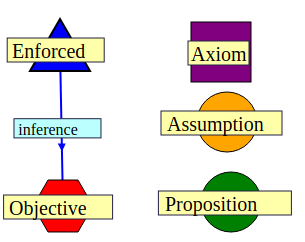
\includegraphics[width=42mm]{legend.png}\ \\
		\caption{Legend for Inference graphs}\label{legend}
\end{figure}

\section{Examples}\label{examplesec}

\subsection{A parcel box}

Consider a box for delivering parcels which can be opened only by the owner and those delivering parcels

The objectives of the system as a whole are:
\begin{itemize}
\item Deliverers are able to store delivered goods in the box whenever they visit the
property with an item to be delivered.
\item Goods can not be taken from the box except by the owner(s) of the box or their agents.
\item The owner of the box is fully informed concerning any deliveries to or removals
from the box.
\end{itemize}


The objective, assumptions, and enforced conditions for this example are listed
in Table \ref{parcelrules}.
\begin{table}[tb]
\centering
\caption{Rules for a parcel box}\label{parcelrules}\ \\
\begin{center}
\begin{tabular}{|c|p{6cm}|}
\hline
\bf Rule Name&\multicolumn{1}{|c|}{\bf Details}\\
\hline
O1 & Parcels cannot be stolen (taken from the box by someone other than the owner) from the parcel box\\
O2 & Parcels can be retrieved from the parcel box by the owner of the box\\
O3 & Deliverers are able to store delivered goods in the box whenever they visit the
property with an item to be delivered\\
A1 & The owner of the parcel box does not allow access to the codes they receive to anyone else\\
E1 & Codes are sent by a secure path to the owner of the parcel box\\
E2 & Codes are sent by a secure path to the parcel box\\
E3 & Codes for access to the box are generated and stored on the server in a system that does not 
provide read access to any person, agent, or process, except for a process that sends them to the owner 
of the parcel box, and to deliverers, and this process cannot be used to send the codes to anyone else\\
E4 & Parcels cannot be removed from a locked box without a code for opening it\\
E5 & Parcels can be removed from a locked box by anyone with the code for opening associated with the parcel it contains\\
E6 & The parcel box can be opened by the code sent to a deliverer, when, and only when, it is empty.\\
E7 & Deliverers are scheduled to visit the parcel box only when it is empty.\\
\hline
\end{tabular}
\end{center}
\end{table}

The inference graph for these rules is shown in Fig. \ref{parcelboxrules}.
\begin{figure}[bhpt]
	\begin{centering}
		\leavevmode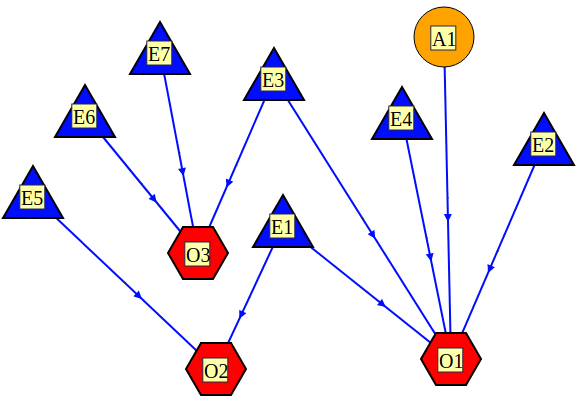
\includegraphics[width=8cm]{parcelboxrules3.png}\ \\
		\caption{Inference graph of rules for a parcel box}\label{parcelboxrules}
	\end{centering}
\end{figure}

This example illustrates the way in which assumptions can, and should, influence the design of a system. If we assume that deliverers can be trusted implicitly, there is no need to ensure that deliverers can only open a parcel box when it is empty. If, on the other hand, we do not make this assumption, the system will need to ensure that deliverers cannot open a parcel box that contains a parcel. This approach is more secure, but a little more difficult to manage. In the past, assuming that deliverers can be implicitly trusted would not seem unreasonable, but in future, as the range of delivery options increases, such an assumption might come to seem unnecessary and unrealistic.

{\em The decision to schedule deliveries to take place only when the parcel box is empty
was made, in the development of this system, in conjunction with, and under the influence
of the cybersecurity inference graph. Objective O1 could be ensured by {\em assuming that
deliverers can be trusted}, but a significantly better design results by searching for 
an alternative to this risky assumption.}

\subsection{A password reset system}
Consider a portal which maintains accounts for users of its services and which has a {\em password reset service}, such as discussed in \cite{exptsandproofs}. The rules which apply to the stakeholders of a service for which a password reset service is available are listed in Table \ref{pwresetrules}.
\begin{table}[tb]
\caption{Rules for the tickets in a password reset system}\label{pwresetrules}
\begin{center}
\begin{tabular}{|c|p{6cm}|}
\hline
		\bf Rule Name&\multicolumn{1}{|c|}{\bf Details}\\
\hline
O1 & Users are able to reset their password by receiving a ticket by email and using this ticket 
at the website within 30 minutes, assuming that they provide an incorrect ticket at most twice.\\
O2 & Agents/persons other than a valid user cannot use this system to reset the password of a user.\\
A1 & Ticket's sent to users are received by email within 1 minute.\\
A2 & Only persons/agents who know a user's email password can access email sent to the user within
the last 30 minutes.\\
A3 & The user's password cannot be guessed.\\
A4 & The user is the only person/agent who knows their email password.\\
A5 & The possibility of an attacker intercepting a ticket on
the user's email client, during its 30 minutes of valid life is negligible.\\
A6 & The possibility guessing a ticket in fewer than 10,000 attempts is negligible.\\
A7 & The server administrator never acts in a way to subvert the intentions of the system he/she administers.\\
E1 & Use of an invalid ticket to reset a password three times or more in 10 minutes, for
a certain user, causes any outstanding tickets for that user to become invalid.\\
E2 & Tickets supplied 31 minutes after generation are no longer valid.\\
E3 & When a ticket is successfully used, it will not be valid in future.\\
E4 & If a user supplies a valid ticket, at the service website, they can use this site to set their password to 
a new setting, without knowing the existing password.\\
E5 & Any user can cause a ticket to be generated and sent to the user's previously registered email address, by 
appropriate actions at the service website.\\
E6 & The {\em only way} to reset a password is by supplying a valid password reset ticket.\\
E7 & The {\em only way} to generate a password reset ticket is by the password
reset service.\\
E8 & Password reset tickets cannot be accessed by any user other than the administrator, on the server
where they are generated.\\
\hline
\end{tabular}
\end{center}
\end{table}

\begin{figure}[bhpt]
	\begin{centering}
		\leavevmode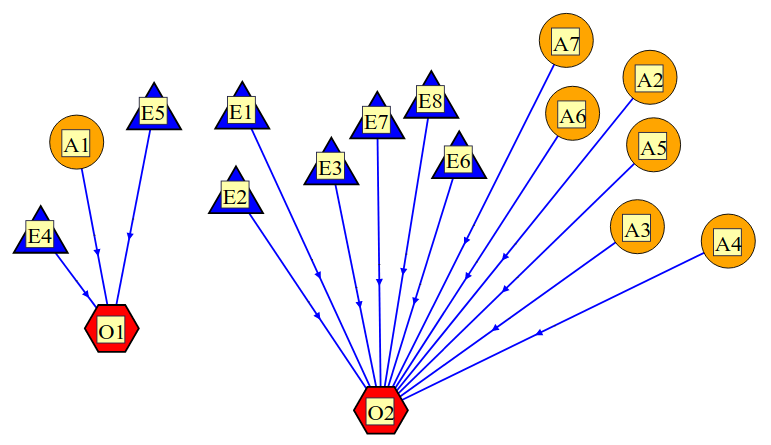
\includegraphics[width=8cm]{pwreset.png}\ \\
		\caption{Inference graph of rules for a password reset system}\label{pwresetrules}
	\end{centering}
\end{figure}

The key requirements for this system are O1 and O2 in this table, i.e. the service can be used to change passwords, but users can only change passwords for {\em their own} accounts. Such systems are vulnerable to logical errors, as discussed in \cite{exptsandproofs}. An inference graph for this system, which can be used to guide its validation, is shown in Fig. \ref{pwresetrules}.


\iffalse
A detail not mentioned in Section \ref{initial} is that when an attempt
to update a user's password is made, with an invalid ticket, the web 
page which is prepared to report an error includes both the invalid
ticket, and the value that the ticket should have taken. This is a fatal
mistake (from the point of view of good security). There is no need
to report to an ordinary user what the value of the ticket should
have been. The reason this was included in the error-report web page
was to enable the software to be readily tested and debugged. However,
this information should have been removed from the error page
in the working system.

The procedure used to change the password of a different user was as
described in Fig. \ref{seqdgnetmlattack}. First, the password reset system was used to reset the password
of the attacker (a perfectly valid procedure, with no ill intent or 
consequence). During this process, the URLs used at each stage
were observed. In particular, the URL which was used to complete
the reset of the password of user \verb|addie11| was of the form
shown in Listing \ref{registration}.
\begin{listing}{\scriptsize
		\begin{minted}[breaklines]{text}
		https://netml.usq.edu.au/netml4_6/registration.jsp?
		resetpwd=true&ticket=12345&uname=u1047621&fullName=fake&
		email=u1047621@umail.usq.edu.au&organisation=USQ
		\end{minted}
	}
	\caption{Form of URL which causes the password change web page to be displayed}
	\label{registration}
\end{listing}
A URL of this form was then used with the target user's email address and 
an invalid ticket. This generated an error report page which revealed
the value the ticket should have had. Finally, the correct ticket was
inserted into the URL and it was sent to the server. This URL caused
the web page for supplying a new password to be displayed, which was then
used to change the target user's password.
\subsubsection{Second Experiment}
After this defect was corrected, by removing the display of the valid ticket on the error report web page,  another experiment was carried out. In some cases, the algorithm used to generate tickets is known by attackers because the source code for the server may be available or the attackers may be able to guess the ticket algorithm \cite{wang2018end}. In the revised Netml system, tickets were calculated as:
\begin{minted}[breaklines]{java}
hexsha(username+Calendar.getInstance()
.get(Calendar.DAY_OF_YEAR))
\end{minted}
In the present case, this algorithm was deliberately revealed to the attacker.

In response to this attack, the ticket algorithm was changed to that shown in Listing \ref{ticketalg}. No attacks of the sort
described in this section were then able to succeed. A proof that these types of attacks can't succeed is given in Section \ref{proof}. 
\fi

\subsection{Signatures}
The validity of the signature of
a document can be checked by the digital signature algorithm.
Once this checking has been done, we can be confident that a person
who has, in their posession, the private key of a certain digital certificate
signed the document. 

What is being checked here is not that the signer is the author, but that they 
are the signer, of the document. Suppose we want to check that Joan is a signatory
of a certain document, {\tt d}. It is not sufficient to merely check the signature,
with the document, and a certain certificate. The validity of the signature also needs
to be checked, and this in turn requires additional checks.
A proof of the statement ``Joan is a valid signatory of document {\tt d}'', which undertakes
all these needed checks, is illustrated in Fig. \ref{certificaterulesgraph}. 
The rules which are used, in this checking process, are described in Table \ref{Authorship}.

With the help of the predicates in Table \ref{certificatepredicates} and the names
of the objects listed in Table \ref{joanobjects}, the 
axioms, listed informally in Table \ref{Authorship}, can now be written, more formally as follows:
\begin{itemize}
		\item[A1:]\label{A1a} 
$\forall A, c, s, ac:\hbox{\tt IsValidAuthority}(A,ac) \wedge \hbox{\tt HasSig}(c,s) \\
	\wedge \hbox{\tt IsValidAccTo}(s,ac,A) \supset \hbox{\tt IsValidCert}(c)$.
	\item[A2:] $\forall A, d, c, s: \hbox{\tt HasCert}(A,c) \wedge \hbox{\tt HasSig}(d,s) \\
	\wedge \hbox{\tt IsValidCert}(c) \wedge$\\
${\tt IsValidAccTo}(s,d,c) \supset \hbox{\tt IsSignatory}(d,A)$.
	% \item[A3:] 
% $\forall A, c: \hbox{\tt HasCert}(A,c) \wedge \hbox{\tt IsValidCert}(c) \supset \hbox{\tt IsValidAuthority}(A)$.
	\item[A3:] $\hbox{\tt IsValidAuthority}(\hbox{\tt VA},{\tt vc})$.
	\item[A4:] $\forall A, c:\hbox{\tt HasCert}(A,c) \wedge \hbox{\tt IsValidCert}(c) \supset \hbox{\tt IsValidAuthority}(A,c)$.
\end{itemize}

Notice that Axiom A4 asserts that {\em anyone} with a valid certificate is a valid authority. 
In a more detailed account, certificates need to include a list of specific capacities that are
granted by the certificate, which will then allow some certificates to empower their owners to
sign other certificates, as well as documents, and others to only sign documents. This feature of
certificates has been omitted from this example in the interest of simplicity.

\begin{table}[tb]
		\caption{Rules for signatures}\label{Authorship}
	\begin{center}
			\begin{tabular}{|c|p{6cm}|}
			\hline
			\bf Rule Name&\multicolumn{1}{|c|}{\bf Details} \\
			\hline
O1& Joan is a valid signatory of document {\tt jdoc}.\\
E1& The document {\tt d} has signature {\tt ds}.\\
E2 & Document {\tt d} is valid according to the digital signature {\tt ds},which uses certificate {\tt jc}\\
E3& Joan has certificate {\tt jc}.\\
E4& The certificate {\tt jc} has signature {\tt jcs}.\\
E5& Certificate {\tt jc} is valid according to signature {\tt jcs} which uses certificate {\tt cc} \\ % & IsValidAccTo(jcs,jc,cc) \\
					E6& {\tt CA} has certificate {\tt cc} \\ % & HasCert(CA,cc)\\
					E7& {\tt cc} has signature {\tt cs} \\ % & HasSig(cc,cs)\\
					E8& {\tt cc} has signature {\tt cs} which is valid according to certificate {\tt vc}\\ % & IsValidAccTo(cs,cc,vc)\\
					% E9& {\tt vc} is a certificate of {\tt VA}\\
					A1& If {\tt A} is a valid authority, {\tt c} is a certificate with signature {\tt s} and the signature {\tt s} is
					valid according to {\tt A}, then {\tt c} is a valid certificate.\\
					A2& If {\tt A} has certificate {\tt c}, {\tt d} has signature {\tt s}, certificate {\tt c} is valid and the signature {\tt s} is
					valid according to {\tt c}, then {\tt A} is a signatory of {\tt d}.\\
					A3& {\tt VA} is a valid authority with certificate {\tt vc}\\
					A4& If {\tt A} has certificate {\tt c} and {\tt c} is valid, then 
					{\tt A} is a valid authority with certificate {\tt c}\\
					P1& {\tt cc} is a valid certificate.\\
					P2& {\tt CA} is a valid authority with certificate {\tt cc}.\\
					P3& {\tt jc} is a valid certificate.\\
			\hline
		\end{tabular}\ \\
	\end{center} 
\end{table}

\begin{table}
\centering
\caption{Predicates used to validate signatures}\label{certificatepredicates}
\begin{tabular}{|@{\tt}l@{\hspace{5mm}}|p{4.5cm}|}
\hline
\bf Predicate&\bf Meaning\\
\hline
HasSig(x,y)& $x$ is a document and $y$ is its signature\\
IsValidAccTo(x,y,z)& $x$ is a signature for document $y$ which is valid according to certificate $z$\\ 
IsSignatory(d,A)& $A$ is a signatory of the document $d$\\
HasCert(A,c)& $c$ is a certificate owned by $A$\\
IsValidCert(x)& $x$ is a valid certificate\\
		IsValidAuthority(X,xc)& $X$ is a valid a certificate authority with certificate {\tt xc}\\
\hline
\end{tabular}
\end{table}

\begin{table}
\centering
\caption{Names of objects and entities which appear in the proof that Joan is the signatory of the document}\label{joanobjects}
\begin{tabular}{|@{\tt}l@{\hspace{2mm}}|p{45mm}|}
\hline
\bf Name&\bf Description\\
\hline
CA& Certisign digital certificate authority\\
VA& Verisign\\
cc& The certificate owned by Certisign which authorizes them as a certificate signing authority\\
jc& Joan's certificate\\
ds& The signature on Joan's document\\
jdoc& The document of Joan\\
\hline
\end{tabular}
\end{table}

Some key objects which are referenced by name in Table \ref{Authorship} are
listed, with their explanations, in Table \ref{joanobjects}. When the informal
statements listed in Table \ref{Authorship} are stated in formal logic we need
to use certain {\em predicates}, the definitions of which are provided in Table \ref{certificatepredicates}.





\subsection{A proof}
Let us now review the proofs of P1, P2, P3 and O1.
Note that although these proof are conceptually simple, 
actually finding them and including all details is not
so easy, and the proofs given here required several iterations,
due to the discovery of logical flaws present in the first attempts.
Such logical flaws can be the basis for attacks if they are not 
discovered by software developers. 
In cases where the need for absolute rigour
is paramount, finding all the details required for a proof to be algorithmically
verified may be warranted.

{\em Finding the proofs of all the propositions and objectives in
this example was achieved with the aid of the inference graph of
their relationships.}

{\bf Proof of P1}


To prove that a certificate is a valid, we can use Axiom A1
with {\tt VA} in place of {\tt A}, {\tt cc} in place of {\tt c}, 
{\tt vc} in place of {\tt ac}, 
and {\tt cs} in place of {\tt s}.
The process of generating a specific version of an axiom in this way
is a feature of the predicate calculus which is needed here and explains
why we need the predicate calculus, not just the propositional calculus,
to correctly model the logic of this system. With these substitutions,
Axiom A1 becomes:
\begin{eqnarray}\label{A2specific}\label{A1special}
&&	\hbox{\tt IsValidAuthority}({\tt VA},{\tt vc}) \wedge \hbox{\tt HasSig}({\tt cc},{\tt cs}) \\ 
&&\wedge \hbox{\tt IsValidAccTo}({\tt cs}, {\tt vc}, {\tt VA} ) \nonumber
\supset \hbox{\tt IsValidCert}({\tt cc}).
\end{eqnarray}
The antecedent conditions of this specialized axiom are
A3, E7 and E8. Two of these conditions are {\em enforced}, and the other is
an axiom. Hence the conclusion of (\ref{A1special}) follows, which
is what we wished to prove.

\begin{figure}[bhpt]
	\begin{centering}
		\leavevmode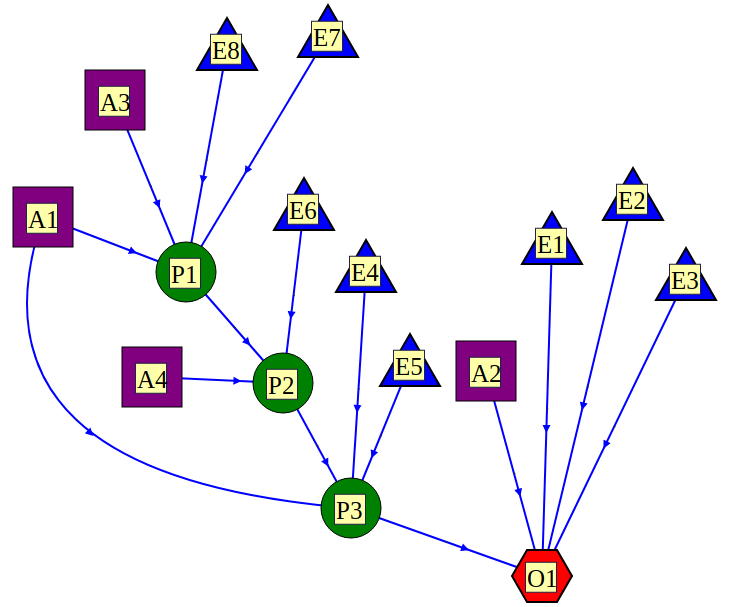
\includegraphics[width=8cm]{rigorous_certificate.png}\ \\
			\caption{Graph of cybersecurity rules and their interdependencies for 
			proof that Joan is a signatory of document {\tt d}}\label{certificaterulesgraph}
	\end{centering}
		\vspace{-5mm}
\end{figure}

\iffalse
\begin{figure}[bhpt]
	\begin{centering}
		\leavevmode\includegraphics[width=8cm]{diagramCyse2.png}\ \\
		\caption{A graph of cybersecurity rules, showing their statements}
	\end{centering}
\end{figure}
\fi

{\bf Proof of P2}

This follows from A4, with P1 and E6 to confirm the antedent conditions.

{\bf Proof of P3}

To prove that  certificate {\tt jc} is a valid, we can use Axiom A1 again
this time with {\tt CA} in place of {\tt A}, {\tt jc} in place of {\tt c}, 
{\tt cc} in place of {\tt ac}, 
and {\tt js} in place of {\tt s}.
With these substitutions,
Axiom A1 becomes:
\begin{eqnarray}\label{A2specific2} \nonumber
&&	\hbox{\tt IsValidAuthority}({\tt CA},{\tt cc}) \wedge \hbox{\tt HasSig}({\tt jc},{\tt js})\\ \nonumber
&&\wedge \hbox{\tt IsValidAccTo}({\tt js}, {\tt cc}, {\tt CA} ) 
\supset \hbox{\tt IsValidCert}({\tt jc}).
\end{eqnarray}
The antecedent conditions of this specialized axiom are
P2, E7 and E8. Two of these conditions are {\em enforced}, and the other is
an axiom. Hence the conclusion of (\ref{A1special}) follows, which
is what we wished to prove.

{\bf Proof of O1}

To prove that an author is a signatory, we can use Axiom A2. In the present instance, O1 follows
from A2 with Joan in place of {\tt A}, {\tt jdoc} in place of {\tt d}, 
{\tt ds} in place of {\tt s}, and {\tt jc} in place of {\tt c}.
The process of generating a specific version of an axiom in this way
is a feature of the predicate calculus which is needed here and explains
why we need the predicated calculus, not just the propositional calculus,
to correctly model the logic of this system. With these substitutions,
the axiom becomes:
\begin{eqnarray}\label{A2specific}\nonumber
&&\hbox{\tt HasCert}({\tt Joan},{\tt jc}) \wedge \hbox{\tt HasSig}({\tt jdoc},{\tt ds}) \\ \nonumber
&&\wedge \hbox{\tt IsValidCert}({\tt jc}) 
\wedge {\tt IsValidAccTo}({\tt ds},{\tt jdoc},{\tt jc}) \\ \nonumber
&&\supset \hbox{\tt IsSignatory}({\tt jdoc},{\tt Joan}).
\end{eqnarray}
The antecedent conditions of this specialized axiom are
P3, E1, E2 and E3. Three of these conditions are {\em enforced}, and P3 has
already been proved, above. Hence the conclusion of this axiom follows, which
is what we wished to prove.


